\documentclass[10pt]{article}
\usepackage[utf8]{inputenc}
\usepackage{graphicx}
\usepackage{hyperref}
\usepackage{pdfpages}
\usepackage{float}
\usepackage[section]{placeins}
\graphicspath{{../assets/ss/}}

% custom

\usepackage{setspace}
\doublespacing
\usepackage[vmargin=1.0in,hmargin=1.5in]{geometry}
\usepackage{pxfonts}
\usepackage{xcolor}
\usepackage{hyperref}
\hypersetup{
    colorlinks,
    linkcolor={black!50!black},
    citecolor={black!50!black},
    urlcolor ={black!50!black}
    }

\title{ 
  Project Report On \\  Paper (An Online Exam Management System)
}

\author{
    \textsc{Sania Rahman}\\
    \small\emph{2017831051}\\

    \textsc{Mehedi Hasan Shifat}\\
    \small\emph{2017831017}\\\\
}

\date{20th Feb,2021}

\begin{document}

\maketitle

\pagebreak

\tableofcontents
% \listoffigures
\pagebreak

\section{Project Introduction}

Technology has changed our lives.Now a days technology has gone so far that everything is online.But our examination system is still dependent on offline activities.This project is about an online web platform where we will be able to init some robust changes to enrich our examination system.


\section{Project Background}

Coronavirus Disease (COVID-19) outbreak poses serious concerns to global education
systems. Efforts to contain COVID-19 prompted unscheduled closure of schools in more
than 100 countries worldwide. COVID-19 school closures left over one billion learners
out of school.
Most governments around the world have temporarily closed educational institutions in an attempt to reduce the spread of COVID-19. As of 30 September 2020,
approximately 1.077 billion learners are currently affected due to school closures in
response to the pandemic.
As a result Online learning has become a critical lifeline for education, as institutions
seek to minimize the potential for community transmission. Technology can enable
teachers and students to access specialized materials well beyond textbooks, in multiple
formats and in ways that can bridge time and space.
Even if online classes are being held but still exams aren’t clear. As authority is not
willing to take risk of student and teacher’s life. So if there’s a feasible online platform
to take exams, then it’ll be possible to clear and prevent session jam.

\section{Project Description}

An online examination is conducted digitally to evaluate students’ academic knowledge and understanding of the curriculum, along with their ability to use creativity to devise new ideas and solutions.
With the advent of the online examination system, the new method of conducting assessments has come to fore. While the traditional methodology persists, but in place of an examination center, students log into an online system to take the test and share their responses. The evaluation and circulation of results are carried out by the assessor.

Our web based online exam management system is capable of arranging exams and taking tests. We mainly focus on taking CQ and MCQ exams arranged by Teachers.

There are two types of user roles  in our system.

\subsection{Teacher}
A Teacher is the Administration user of our system where teacher will be able to set exams.

\subsubsection{Course Create} Teacher will create course and an automatic invitation will be sent to the students of the department.
\subsubsection{Question Create} Teachers are able to create cq and mcq questions for the exams.
\subsubsection{Exam Create} Teacher will create exam after questions are created and the exam Notification will be sent to all the students assigned in the course.
\subsubsection{CQ Examine} There is a manually cq exam paper checking feature for teacher. Then result of cq will be sent to the student automatically.
\subsubsection{Marksheet Check} Teacher can see all the results of the students and analyse the performance of the students and take necessary steps to make better.
\subsubsection{Feedback Check} Teachers can check the report or feedback of students on every questions.
\subsubsection{Result Print} Teacher can print the marksheet of the specific exam for offline distribution.

\subsection{Student}

Another user is Student. Students will be able to participate in the exams arrranged by Teachers.

\subsubsection{Real-Time Exam} Students will be able to  participate in realtime exam.

\subsubsection{Revise Previous Exam} Students will be able to see the previous exams and questions with answers. If they had attended in the exam then they will also be able to check their wrong answers. It will be helpful for them to check their previous exams.

\subsubsection{Realtime Notifications} Students can get invitation for courses instantly. They will be notify when any exam will be created in their course and the result publication of cq exam will also be notified.

\subsubsection{Feedback} In exam time, if they find something wrong, they can report about it.

\subsubsection{Late Participate}
We have made the online examination system in such a way that students will be able to participate in the exam if they are late. They can submit the answer before the given time on the questions and go to the next one.That's how one can solve all questions even they attend in the exam late.

\subsection{Exam}

The main feature of our application is making the examination system online.In our app student will be able to participate in the exams online set by their teachers.

\textbf{Types of exams :}

\begin{itemize}
  \item Multiple Choice Question (MCQ) Exam

  \item Creative Question (CQ) Exam
\end{itemize}

\subsubsection{Question features}

\begin{itemize}
  \item MCQ and CQ Questions
  \item Specific time limit for each questions
  \item Specific mark set for each questions
  \item Report system for each questions of a exam
\end{itemize}

\subsubsection{Exam Features}

\begin{itemize}
  \item Real-Time exam
  \item Set time and Date for upcoming Exams
  \item Automatic marking system for mcq questions
  \item Manual marking system for cq questions
  \item Secure exam access and answer submission
  \item Countdown clock in examination
  \item Disable copy and paste in question and answer section
  \item Focus change alert in exam time
  \item Instant result show for mcq questions
  \item Realtime Notifications for exams and cq exam results
\end{itemize}

\section{User Interface Specifications}
\subsection{Authentication}
\subsubsection{Signup} First of all any user needs an verified account to use our application. So he need to signup for creating a new account where he have to use his verified email address given by his/her university. Without a valid email address no one will be able to create any user account.The signup information differs from user type to user type.

\begin{figure}[H]
  \centering
  \centerline{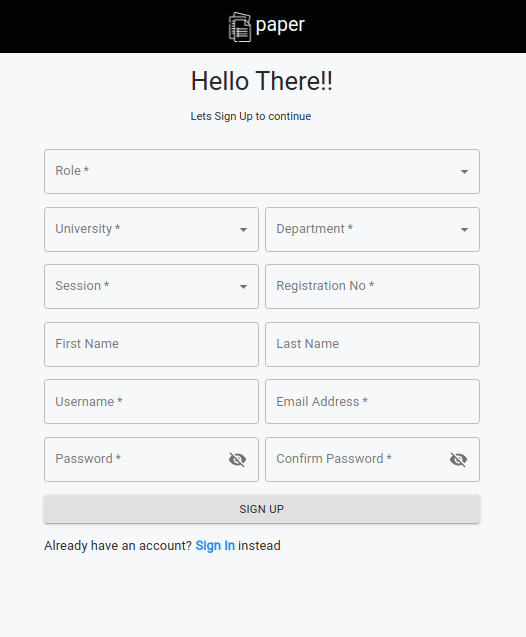
\includegraphics[width=0.6\textwidth]{signup/signup.png}}
  \caption{Signup Page}
  \label{fig}
\end{figure}

System will notify if any errors occurs such as

\begin{itemize}
  \item Email address not authorized
  \item Username already exists
  \item Email address already exists
  \item Password didn't matched
\end{itemize}

\begin{figure}[H]
  \centering
  \centerline{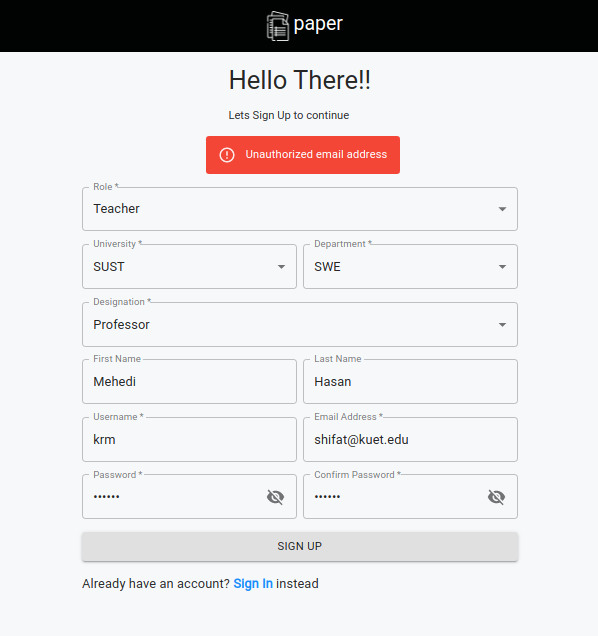
\includegraphics[width=0.6\textwidth]{signup/signup-error-e.png}}
  \caption{Signup Page : Unauthorized email address error}
  \label{fig}
\end{figure}

\begin{figure}[H]
  \centering
  \centerline{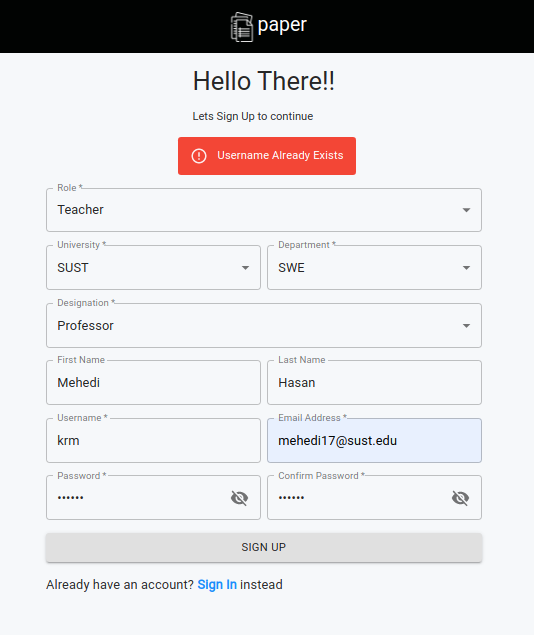
\includegraphics[width=0.6\textwidth]{signup/signup-error-u.png}}
  \caption{Signup Page : Already used username error}
  \label{fig}
\end{figure}


\subsubsection{Login}

When a user has a verified account they can login whenever he/she wish. Our login system.
In order to login, user needs to input his/her email and password.

\begin{figure}[H]
  \centering
  \centerline{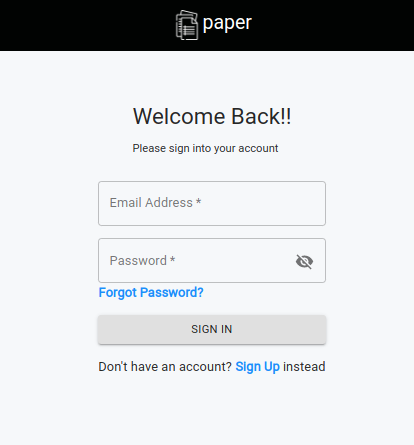
\includegraphics[width=0.6\textwidth]{login/login.png}}
  \caption{Login Page}
  \label{fig}
\end{figure}


Authentication verify and errors show :

\begin{figure}[H]
  \centering
  \centerline{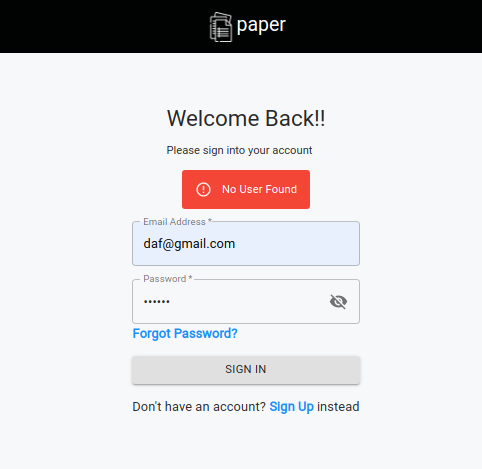
\includegraphics[width=0.6\textwidth]{login/login-error1.png}}
  \caption{Login Page : Invalid email address error}
  \label{fig}
\end{figure}

\begin{figure}[H]
  \centering
  \centerline{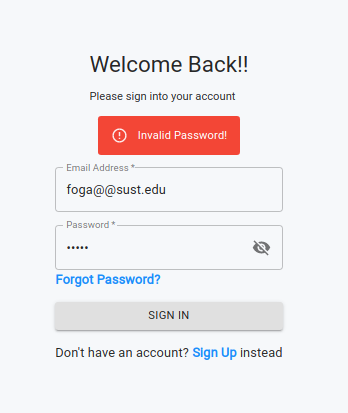
\includegraphics[width=0.6\textwidth]{login/login-error2.png}}
  \caption{Login Page : wrong password error}
  \label{fig}
\end{figure}

\subsection{Home Page}
It is a common page for all users.In home page an authorized user will show three sections.They are -

\begin{figure}[H]
  \centering
  \centerline{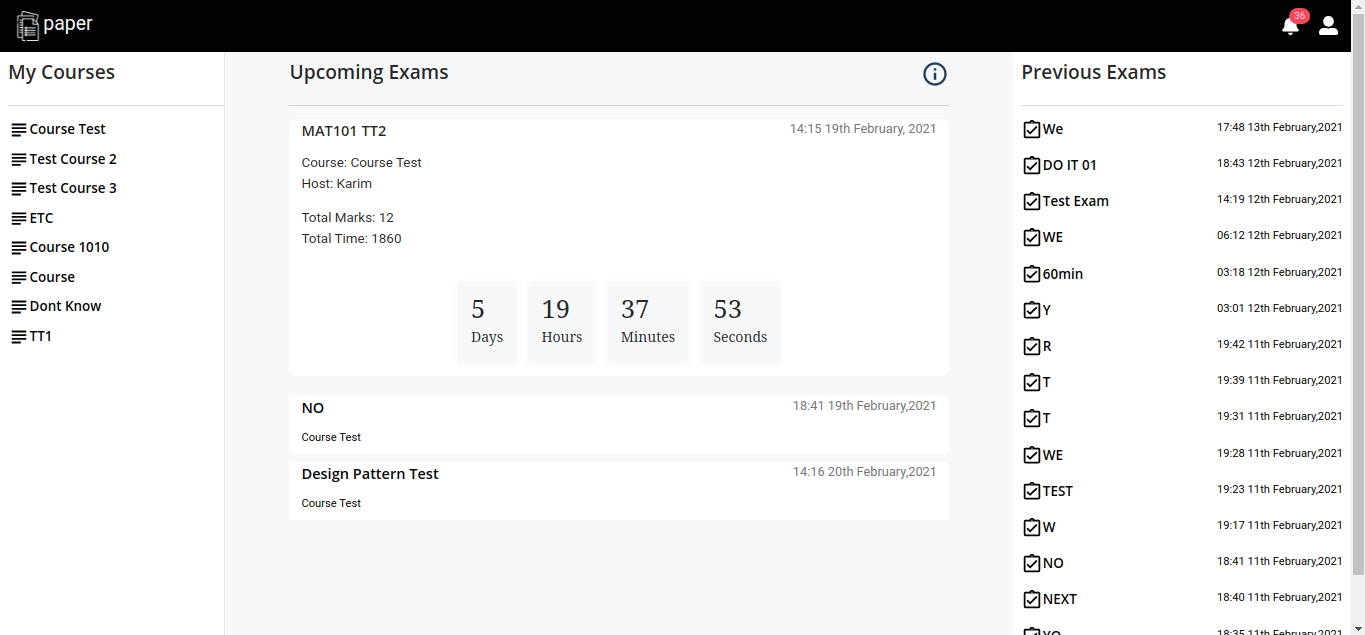
\includegraphics[width=\textwidth]{home.png}}
  \caption{Home Page View}
  \label{fig}
\end{figure}

\subsubsection{Courses}
In course section, user interfaces will be different for different roles users.
The students will see a list of all joined courses where the teacher will see the courses he created and a button to create more courses.

\subsubsection{Course Creation}

Teachers are able to create new courses for the students.

\begin{figure}[H]
  \centering
  \centerline{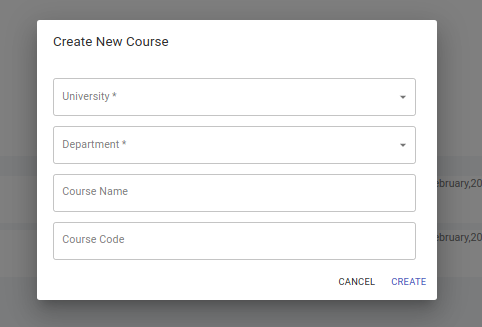
\includegraphics[width=\textwidth]{teacher/course-create.png}}
  \caption{Teacher View: Course Creation}
  \label{fig}
\end{figure}

\subsubsection{Countdown Timer}

At the focus of the home page, there is a Countdown clock to chase the time of most upcoming exam.

\subsubsection{Upcoming Exams}
There is a list of all upcoming exams at the home page.

\subsubsection{Previous Exams}
At the left side of the screen there is a section for all previous exams.

\subsection{Upcoming Exam Page}
Detail information for upcoming exams can be checked in this page.

\begin{figure}[H]
  \centering
  \centerline{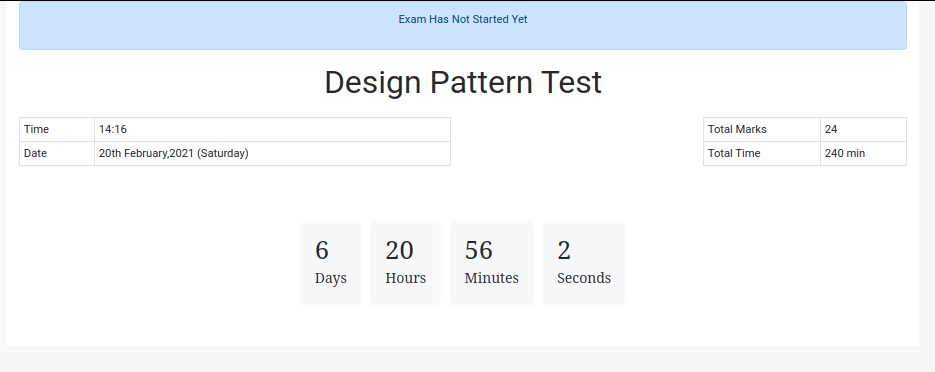
\includegraphics[width=\textwidth]{studnt/upcoming-exam.png}}
  \caption{Upcoming Exam Page}
  \label{fig}
\end{figure}

\subsection{Previous Exam Page}

The user interface of previous exam page is shown differently for a teacher and a student.

\subsubsection{Exam Detail}

Student will be able to see the exam detail info such as

\begin{itemize}
  \item Exam name
  \item Time
  \item Date
  \item Mark
  \item Obtained mark
  \item Participated or not
\end{itemize}

\begin{figure}[H]
  \centering
  \centerline{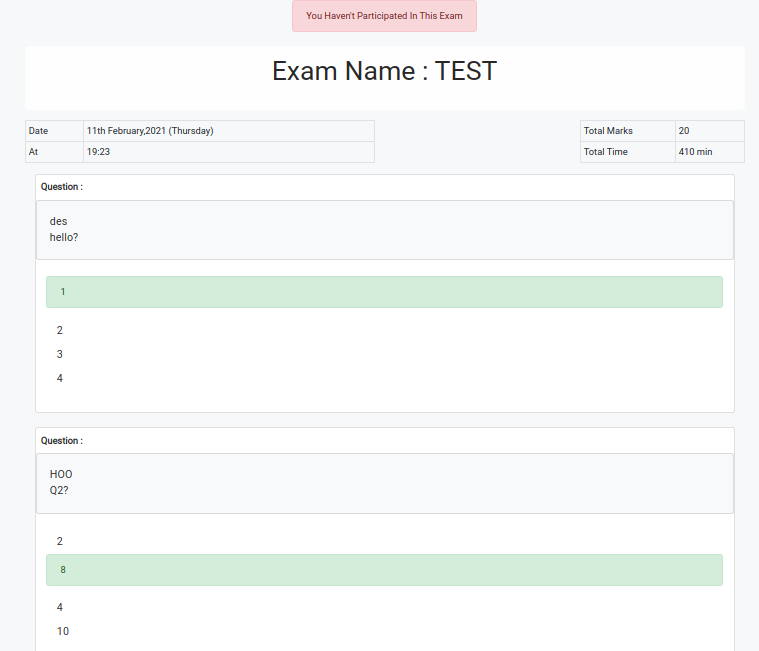
\includegraphics[width=\textwidth,height=0.5\textheight]{studnt/previous-exam-non-participate.png}}
  \caption{Student View : Previous MCQ Exam}
  \label{fig}
\end{figure}

\subsubsection{My Answers}

\begin{figure}[H]
  \centering
  \centerline{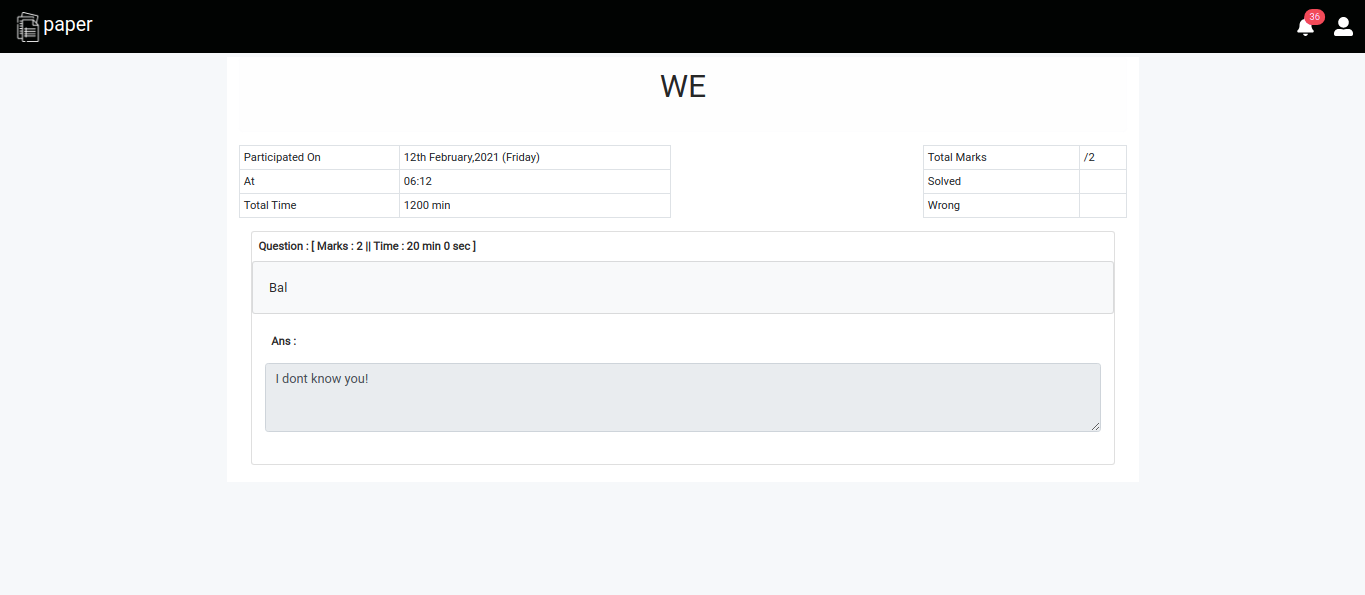
\includegraphics[width=\textwidth]{studnt/previous cq.png}}
  \caption{Student View : Previous CQ Exam}
  \label{fig}
\end{figure}

\subsubsection{Marksheet}

\begin{figure}[H]
  \centering
  \centerline{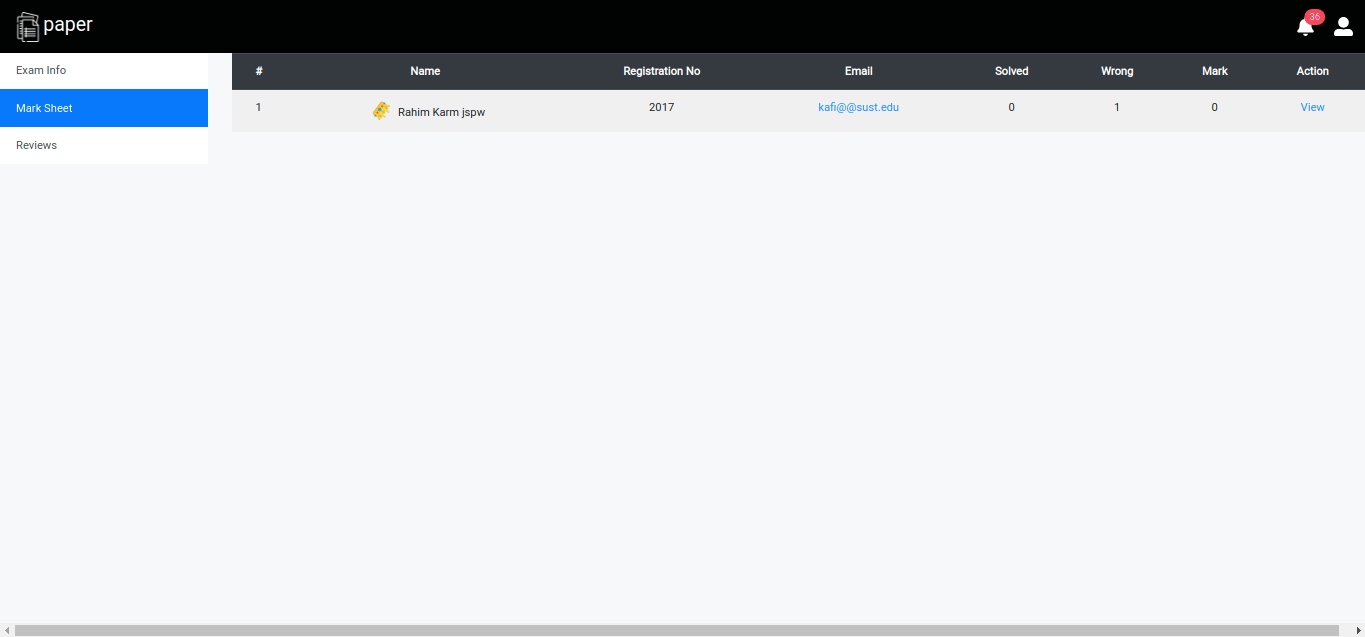
\includegraphics[width=\textwidth]{teacher/marksheet.png}}
  \caption{Teacher View: Marksheet of Exam}
  \label{fig}
\end{figure}

\subsubsection{Reports}

Students are able to report or give feedback about questions while exam. The teacher will be able to see the reports so that he can improve these types of problems.

\subsection{Course Page}


\subsubsection{Course Info}

A Detail information of the course is shown here for the user.

\subsubsection{Exam Creation}

Only the teacher is able to create exam for courses. There are two types of exams a teacher can create.

\begin{itemize}
  \item MCQ
  \item CQ
\end{itemize}

First of all, teacher has to make questions for the exam. Then he set name, time and date  for the exam and confirm it.

\begin{figure}[H]
  \centering
  \centerline{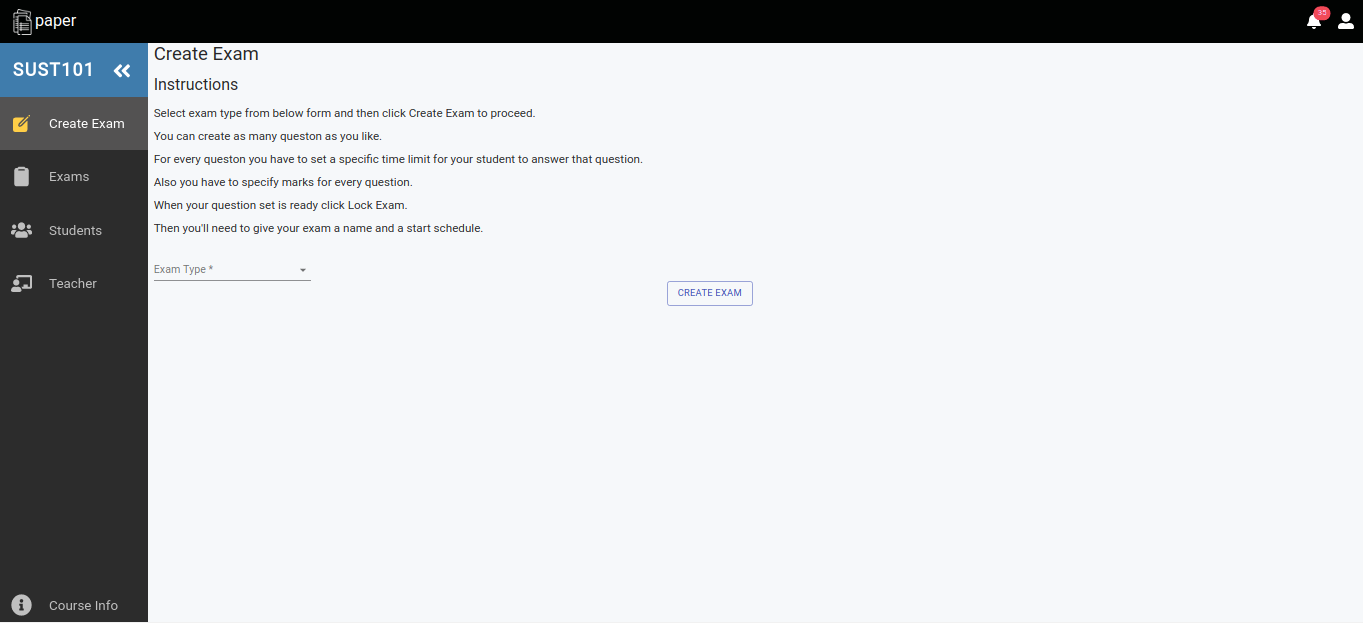
\includegraphics[width=\textwidth]{teacher/exam-create.png}}
  \caption{Teacher View: Exam Type Select}
  \label{fig}
\end{figure}


\begin{figure}[H]
  \centering
  \centerline{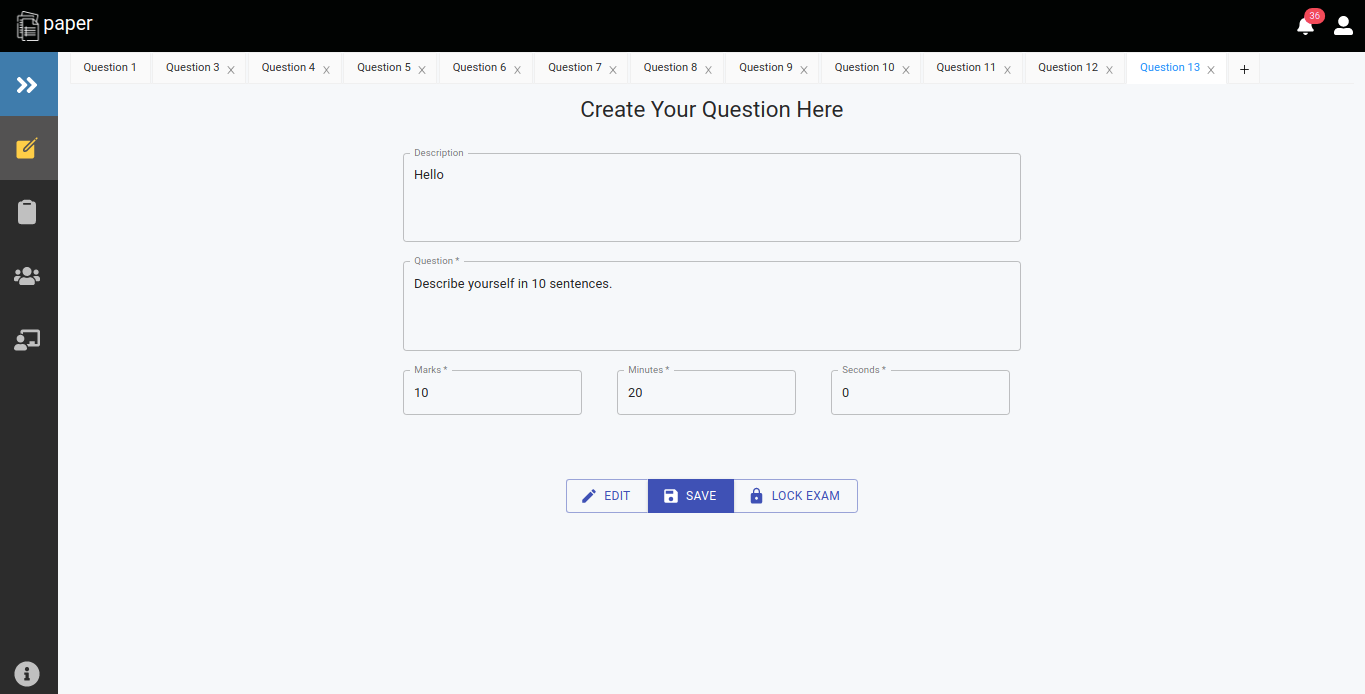
\includegraphics[width=\textwidth]{teacher/cq-create.png}}
  \caption{Teacher View: CQ Question Create}
  \label{fig}
\end{figure}

\begin{figure}[H]
  \centering
  \centerline{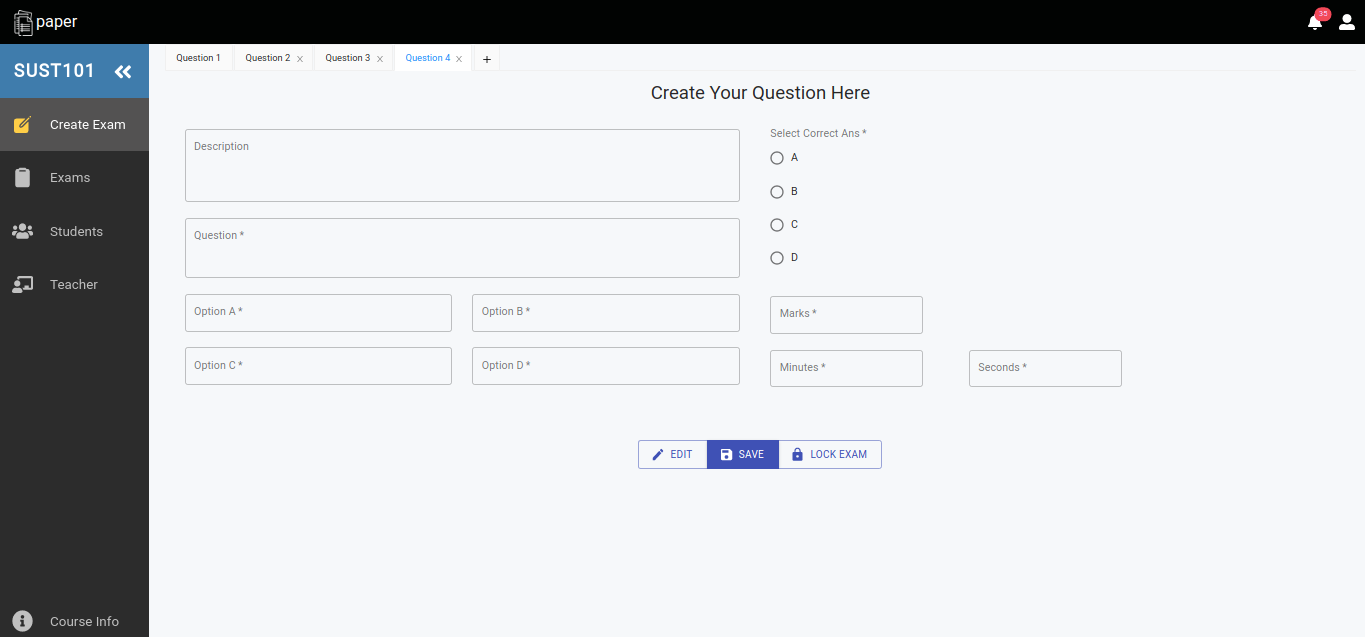
\includegraphics[width=\textwidth]{teacher/mcq-create.png}}
  \caption{Teacher View: MCQ Question Create}
  \label{fig}
\end{figure}

\begin{figure}[H]
  \centering
  \centerline{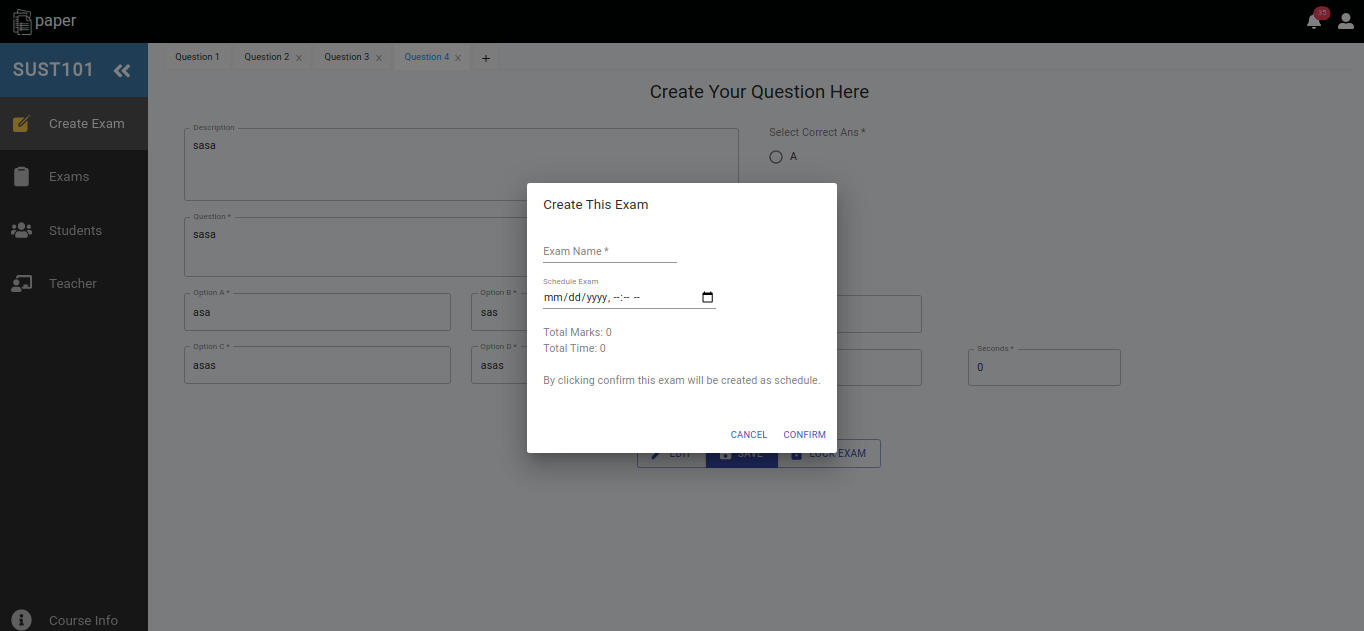
\includegraphics[width=\textwidth]{teacher/set-exam.png}}
  \caption{Teacher View: Exam Creation}
  \label{fig}
\end{figure}

\subsubsection{All Exams}


\begin{figure}[H]
  \centering
  \centerline{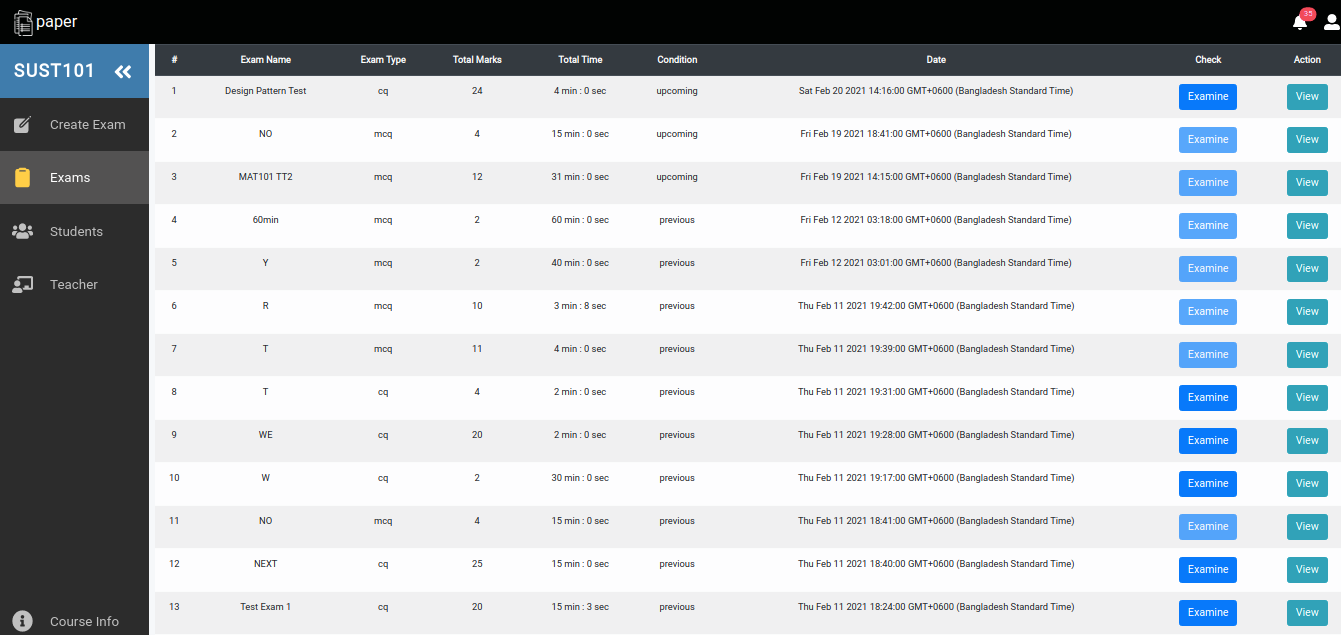
\includegraphics[width=\textwidth]{teacher/all-exams.png}}
  \caption{Course Page : All Exams in the course}
  \label{fig}
\end{figure}

\subsubsection{Students}

A table of all students information assigned in the course are show here so that teacher can overview the students performance.

\subsubsection{Teacher Info}

Students will be able to check the detail information of the teacher who is taking the course.


\subsection{Real-time Exam}

This is an interactive user interface for live exam.

\begin{figure}[H]
  \centering
  \centerline{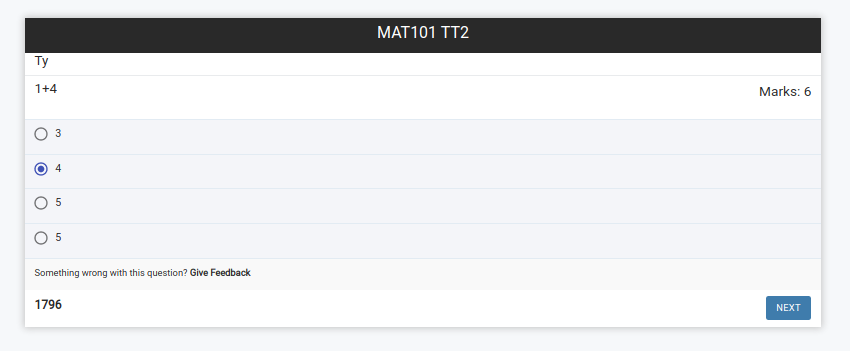
\includegraphics[width=\textwidth]{studnt/live-exam-mcq.png}}
  \caption{Student View: Realtime MCQ Exam}
  \label{fig}
\end{figure}

\begin{figure}[H]
  \centering
  \centerline{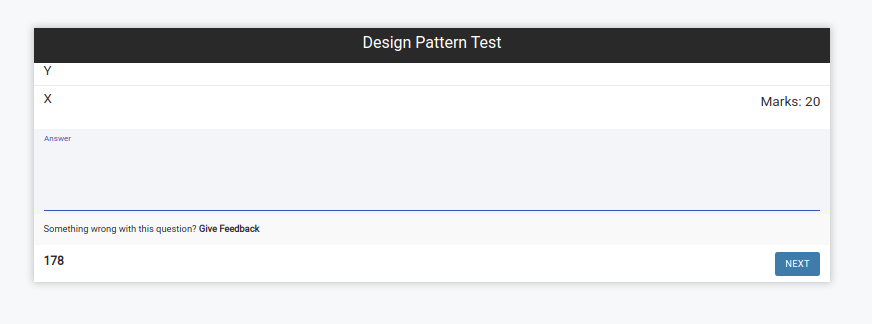
\includegraphics[width=\textwidth]{studnt/live-exam-cq.png}}
  \caption{Student View: Realtime CQ Exam}
  \label{fig}
\end{figure}



\subsection{Examine CQ}

Teacher can check cq exams manually and give mark on them.

\begin{figure}[H]
  \centering
  \centerline{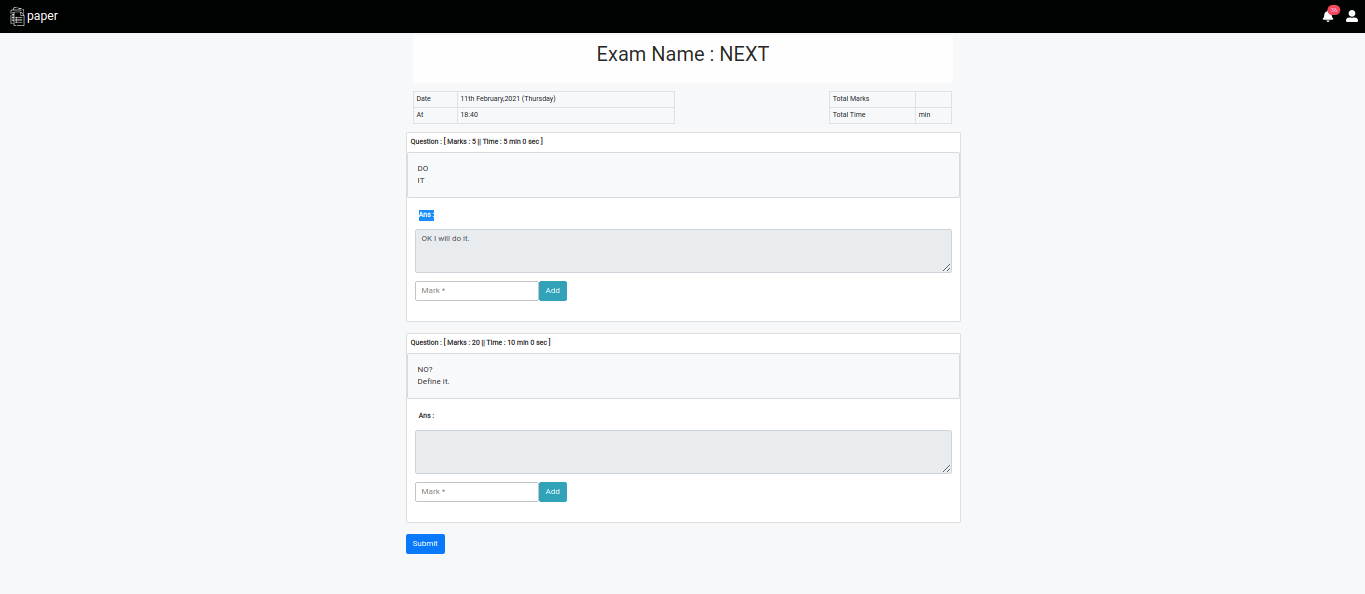
\includegraphics[width=\textwidth]{teacher/examine-cq2.png}}
  \caption{Teacher View: CQ Examine}
  \label{fig}
\end{figure}

\subsection{Notifications}

Users are able to see notifications of -

\begin{itemize}
  \item Course Creation
  \item Exam notifications
  \item CQ result publish
\end{itemize}

\begin{figure}[H]
  \centering
  \centerline{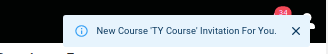
\includegraphics[width=\textwidth]{studnt/course-create-notification-realtime.png}}
  \caption{Realtime Notification :  Course Invitation}
  \label{fig}
\end{figure}

\begin{figure}[H]
  \centering
  \centerline{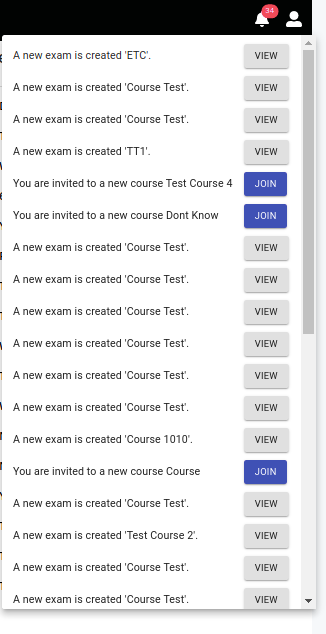
\includegraphics[width=\textwidth,height=0.8\textheight ]{studnt/notifications.png}}
  \caption{Student View: All Notifications}
  \label{fig}
\end{figure}

\section{System Design}

\subsection{Use Case Diagram}

\begin{figure}[H]
  \centering
  \centerline{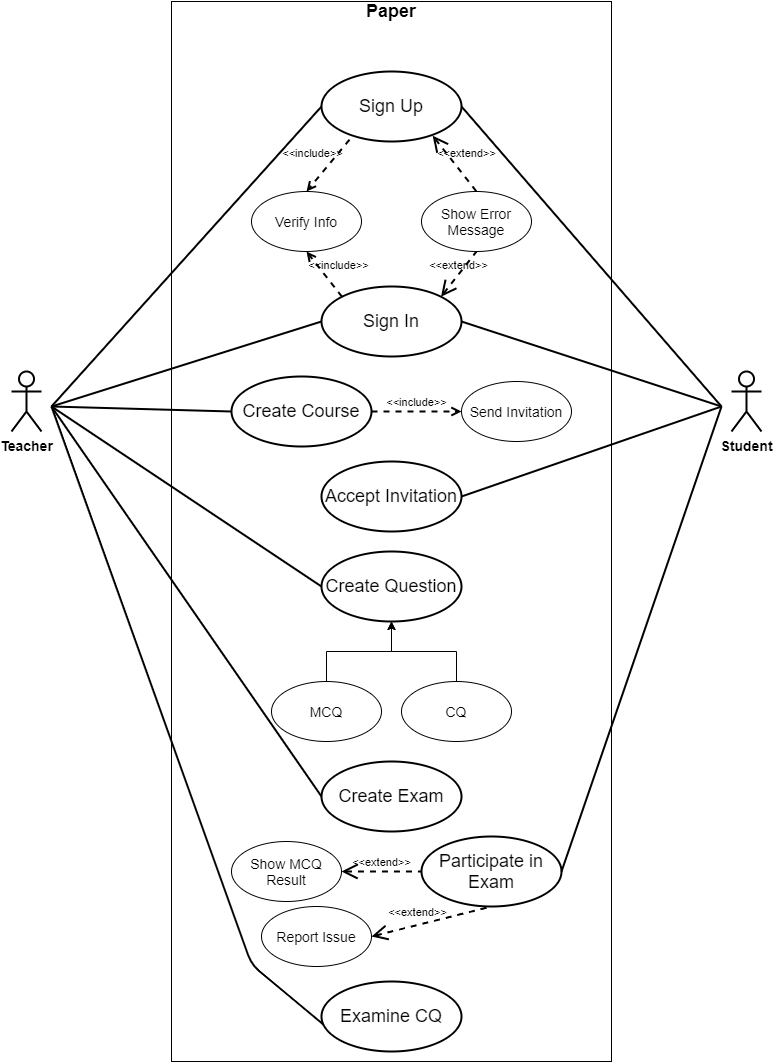
\includegraphics[width=\textwidth]{diagram/level1.png}}
  \caption{Use Case Diagram}
  \label{fig}
\end{figure}

\subsection{Context Diagram}
\begin{figure}[H]
  \centering
  \centerline{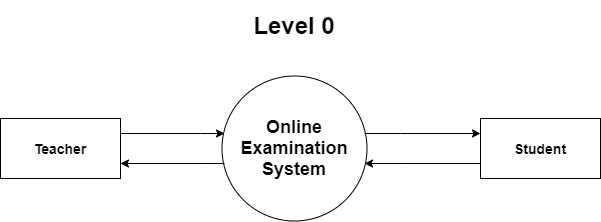
\includegraphics[width=\textwidth]{diagram/level0.png}}
  \caption{Context Diagram}
  \label{fig}
\end{figure}

\subsection{Data Flow Diagram}

\subsection{Entity Relationship Diagram}

\section{System Architecture}

\subsection{Front-End}
In frontend we have used reactjs which is a framework of javascript to design user interfaces.Here we have followed Component Based Architecture.

\subsection{Back-end}

In backend development we created restful api using javascript backend framework Express. We followed Model View Controller (MVC) here.

\begin{figure}[H]
  \centering
  \centerline{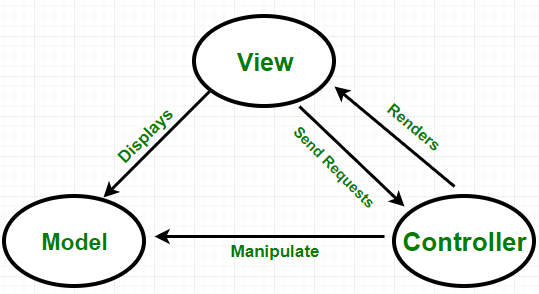
\includegraphics[width=\textwidth]{diagram/mvc.png}}
  \caption{Model View Controller Architecture}
  \label{fig}
\end{figure}


\section{System Implementation}

We can separate the whole system Implementation into two sections.

\begin{itemize}
  \item Frontend
  \item Backend
\end{itemize}

We have used ExpressJs as server side framework for backend-server,React for frontend, MongoDB for database.
The frontend and backend are developed separately and merged through Restful api. We have designed api end-points to fetch data from database to frontend. We have also implemented Sokcet-IO for realtime notification integration.

\begin{figure}[H]
  \centering
  \centerline{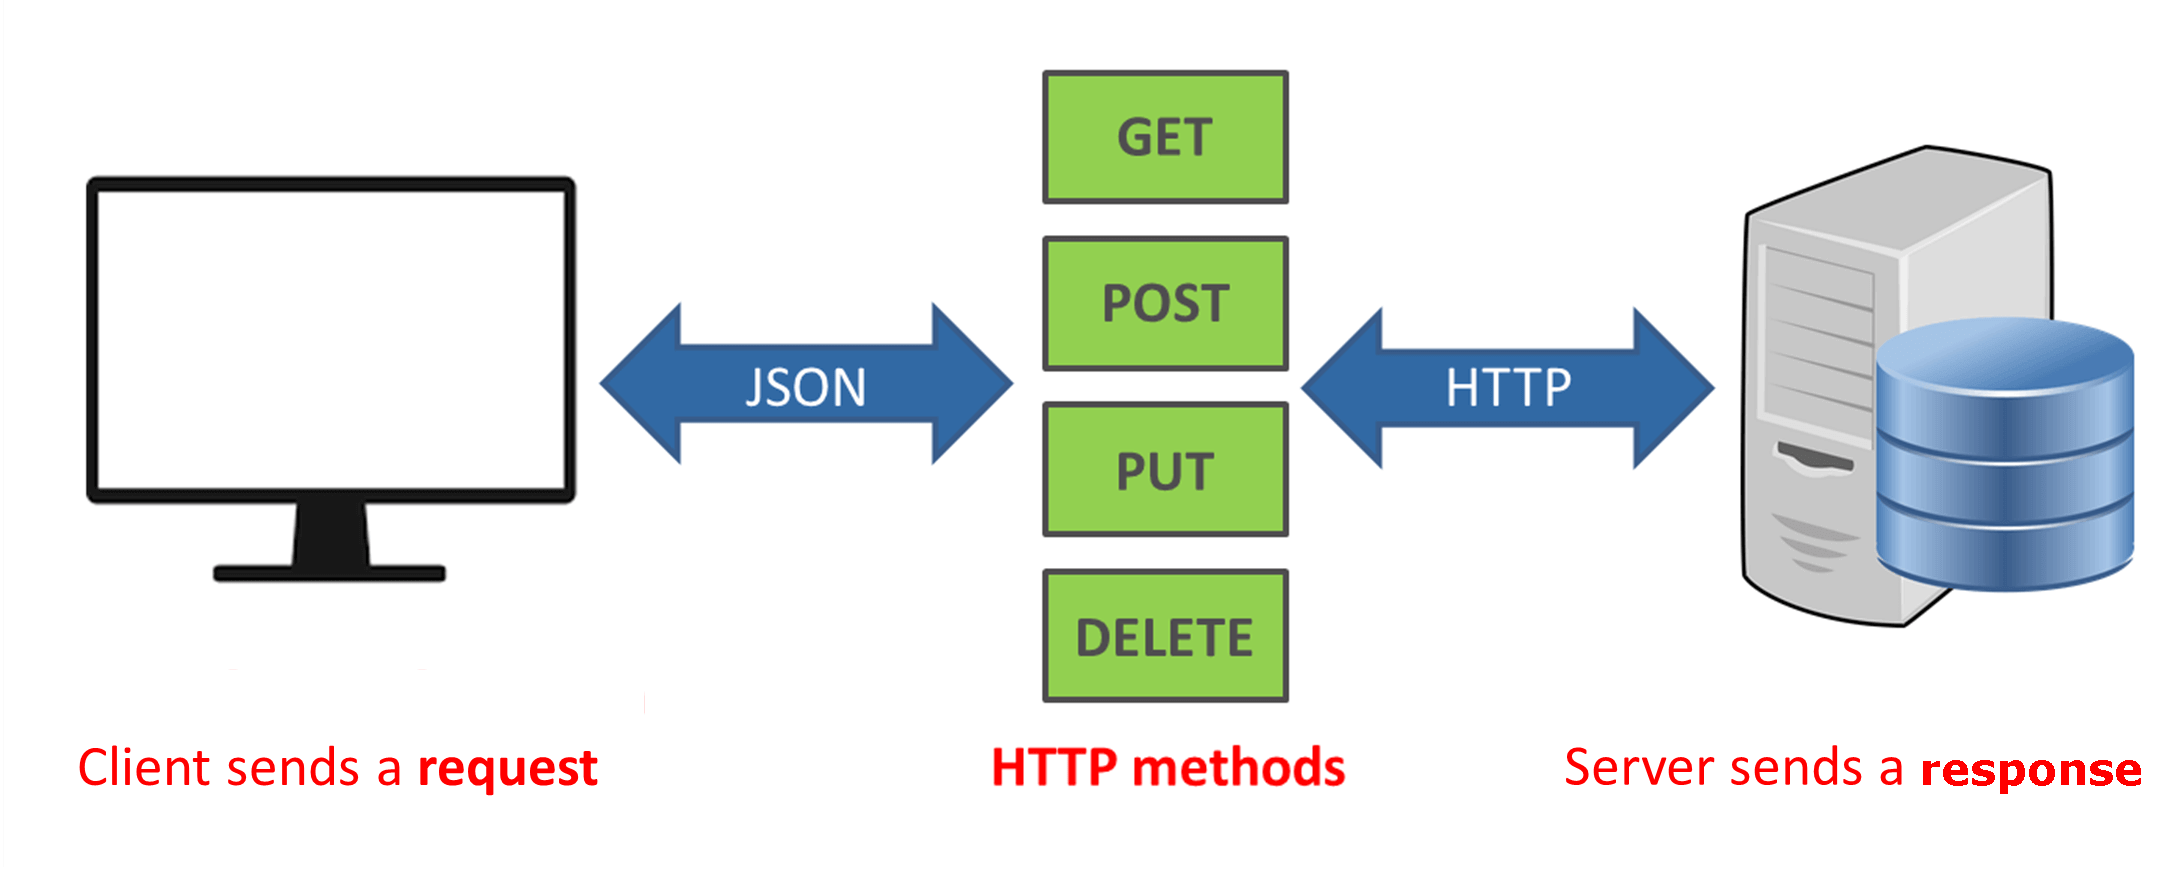
\includegraphics[width=\textwidth]{diagram/api.png}}
  \caption{Backend-Frontend Merged Through API}
  \label{fig}
\end{figure}


\subsection{Authentication}

For authentication we have used Javascript Web Token (jwt). The backend send a token for every users when they login or signup in the frontend. The frontend saves the token and use it everytime it sends request to the server. That's how the system becomes more secure.

\begin{figure}[H]
  \centering
  \centerline{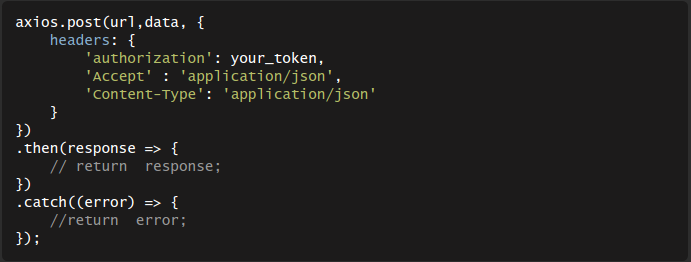
\includegraphics[width=\textwidth]{api-call.png}}
  \caption{Frontend : React Api call with jwt token}
  \label{fig}
\end{figure}

\subsection{Pattern Of Code}

\subsubsection{Frontend}

We have divided the whole system into small components. First we define the components and them merge them with the system.Our component based system :

\begin{figure}[H]
  \centering
  \centerline{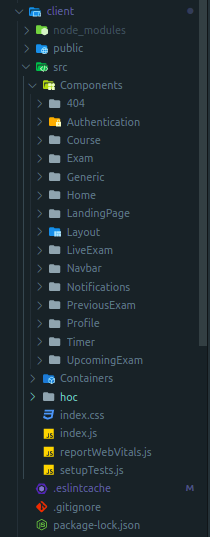
\includegraphics[width=0.5\textwidth]{frontend-components.png}}
  \caption{Frontend components based System Structure}
  \label{fig}
\end{figure}

In frontend we have called api to fetch data from database.

\begin{figure}[H]
  \centering
  \centerline{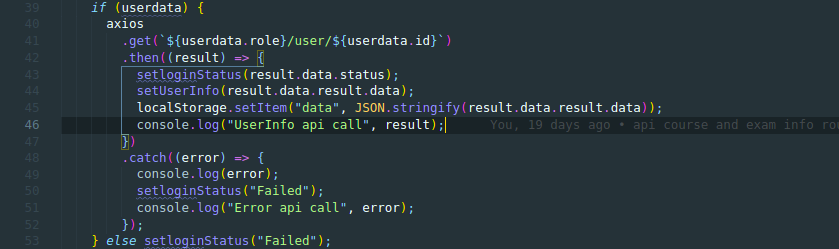
\includegraphics[width=\textwidth]{api-call2.png}}
  \caption{Frontend Api calling}
  \label{fig}
\end{figure}

\subsubsection{Backend}

In backend we have separated the controllers, routes and models.All the end-points and routers are defined in routes folder.The models folders are for database models and controller controls the post and get method and send responses to the frontend.

\begin{figure}[H]
  \centering
  \centerline{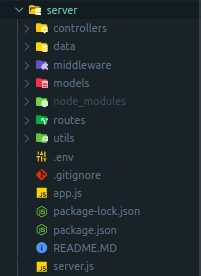
\includegraphics[width=.5\textwidth]{backend.png}}
  \caption{Backend File Structure}
  \label{fig}
\end{figure}

\begin{figure}[H]
  \centering
  \centerline{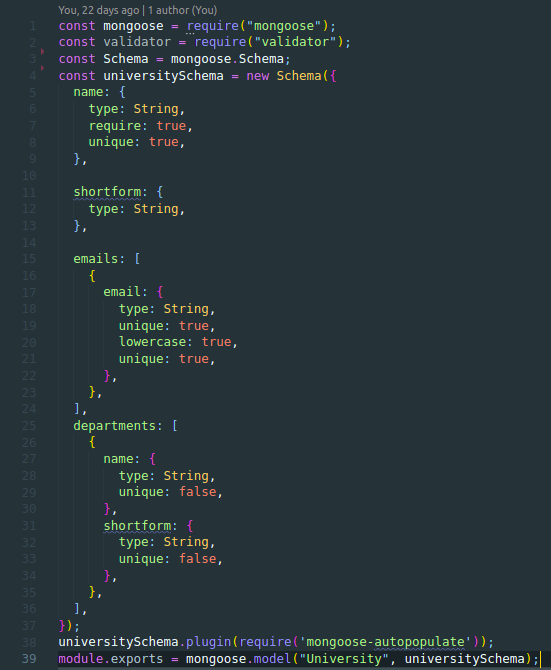
\includegraphics[width=.6\textwidth]{model.png}}
  \caption{Backend : Model Sample}
  \label{fig}
\end{figure}

\begin{figure}[H]
  \centering
  \centerline{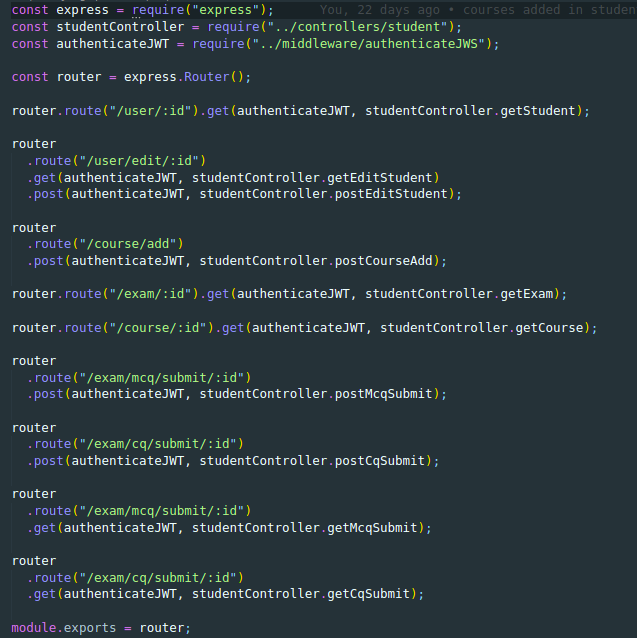
\includegraphics[width=.6\textwidth]{routes.png}}
  \caption{Backend : Model Route}
  \label{fig}
\end{figure}


\section{Testing And validation}

Software Testing is Important because if there are any bugs or errors in the software, it can be identified early and can be solved before delivery of the software product. Properly tested software product ensures reliability, security and high performance which further results in time saving, cost effectiveness and customer satisfaction.

Before releasing the software we have gone through some testing methods to check whether the actual software product matches expected requirements and to ensure that software product is Defect free.
We have classified our testing system into two catagories. They are -
\subsection{Functional Testing}


\subsubsection{Unit Testing : } This is the first stage of testing our system where we divided our  system into several units, functions and components. The purpose is to validate that each unit of the software code performs as expected. Unit Testing was done during the development (coding phase) of an application by our developers. It isolated a section of code and verify its correctness. Thats how we finished our unit testing.

\subsubsection{Integration testing : }

As our project consists of multiple software modules, coded by different programmers so we integrated the modules logically and tested as a group. The purpose of this level of testing is to expose defects in the interaction between these software modules when they are integrated. We focused on checking data communication amongst these modules.

\subsubsection{System testing: }

After Integration testing we  validated the complete and fully integrated software product.The purpose of  system test is to evaluate the end-to-end system specifications.

In system testing we focused on -

\begin{itemize}
  \item \textbf{Usability Testing} - mainly focused on the user's ease to use the application, flexibility in handling controls and ability of the system to meet its objectives.
  \item \textbf{Load Testing} - we tested real-life loading scenarios such as

        \begin{itemize}
          \item Home screen loading
          \item Login, Signup loading
          \item Next pages Loading
          \item Course Join
        \end{itemize}


  \item \textbf{Migration testing} - is done to ensure that the software can be moved from older system infrastructures to current system infrastructures without any issues.
\end{itemize}

\subsubsection{Acceptance Testing : }

This is the final level of testing. In Acceptance testing we determined that this application is ready to release as it meets all the requirements and validations.


\subsection{Non-Functional Testing}

In non functional testing we were testing the non functional requirements of the system such as security, performance, usability, scalability.

\subsubsection{Load Testing}

Our load testing involves testing the system's loading capacity. Loading capacity means more and more people can work on this system simultaneously.

\subsubsection{Security Testing}

The most focus on our system is the security as it is a system to take exams and we ensure the security most. We tested the account creation system so that no unauthorized user will be able to signup in our application. We also tested the exam time verification system too.


\subsubsection{Reliability Testing}

In reliability testing we assure that the system is running without fail under specified conditions and it must be run for a specific time and number of processes.

\subsubsection{Efficiency Testing}

We tested the Efficiency of our system if it becomes slow or not when more users are interacting with our system.


\section{Future Enhancement}

As our project is in a beginning stage, we have plans to add several features in future.  Our plan includes features like -

\begin{itemize}
  \item \subsection{Combined Exams} Currently in our application MCQ and CQ exams are two seperate types of exam. But in future exams can have both CQ  and  MCQ types of questions.
  \item \subsection{Lab Exams} For now our system is able to take theoretical exams  but we are eager to implement lab exams such as coding related course exams online.
  \item \subsection{Realtime Chat} Teachers and students will be able to chat for necessary information. This will reduce communication gaps between them.
  \item \subsection{Mobile Version} We will release our application for mobile users as it will be more easy for students to participate in exam online.
\end{itemize}

\section{Conclusion}

This web based application will make robust changes in our education system.It will help the education system to continute our educational progress during lockdown and COVID-19 pandemic.It will save students from Session jam.

\section{References}

\begin{itemize}
  \item \href{https://journals.plos.org/plosone/article?id=10.1371/journal.pone.0239490}{Influence of COVID-19 confinement on students’ performance in higher education}
  \item \href{https://www.tandfonline.com/doi/abs/10.1080/08941939.2020.1748147?journalCode=iivs20}{The Effects of COVID-19 on Academic Activities and Surgical Education in Italy}
\end{itemize}

\end{document}
